\documentclass[11pt]{jarticle}
%文書クラスを最初に指定.英語なら{article}.
%article は記事用のクラスで文章構造は部 (part)、節 (section)、小節 (subsection)、小小節(subsubsection)、段落 (paragraph)、小段落 (subparagraph) で構成される。通常は section から始めることが多い。
%字を大きくしたかったら [12pt] などとすれば良い.
%Latex ではパーセント(%)記号以降は改行があるまでコメントアウトされる.
\usepackage[dvipdfmx]{graphicx} %図を取り込むのに必要.
\usepackage{amsmath,amssymb} %アメリカ数学会拡張パッケージ
\usepackage{bm} %数式用太字斜体コマンド \bm
%このように、必要な拡張パッケージを \usepackage で有効化することができる

\title{ガウスの法則とアンペールの法則のノート}
\author{名大 太郎}
\date{2022年12月1日}

\begin{document} %本文開始

\maketitle %上記で定義した title, author, date を表示.

\begin{abstract} %概要の始め
ガウスの定理とストークスの定理より,電磁気学のガウスの法則とアンペールの法則の微分形の表式を求める.
\end{abstract} %概要の終わり

\section{ガウスの法則} %第 1 節
\subsection{積分形} %より細かく小節分け.
体積$V$,表面積$S$を持つ領域を考える.%文中の数式は$...$で囲む.
この領域内の電荷$Q$と表面を貫く電場$\bm{E}$には%\bm{}で太字斜体(bmパッケージを利用)
以下の関係が成り立つ.
\begin{equation} %独立数式の初め
  \oint_{\bm{S}} \epsilon_0 \bm{E} \cdot d\bm{S} = \int_{V} \rho_q dV = Q
  % 下添字は_を用いる. ちなみに上添字は^である.
  % \oint は周積分記号, \int は積分記号である.
  % 内積は\cdot. \epsilon や\rho はギリシア文字である.
  \label{eq:integGauss} %式ラベル.別の場所から引用する時に使用.
\end{equation} %数式の終わり
但し,$\epsilon_0$は誘電率,$\rho_q$は電荷密度である.

\subsection{ガウスの定理}
任意のベクトル$\bm{A}$に対して
\begin{equation}
  \int_V \bm{\nabla \cdot A} dV = \oint_{\bm{S}}\bm{A}\cdot d\bm{S}
  \label{eq:divGauss}
\end{equation}
が成り立つ.

\subsection{微分形}
式 (\ref{eq:divGauss}) を電場$\bm{E}$に適用し,式 (\ref{eq:integGauss}) と比較すると
%\ref により上記で定義した式番号を引用.
\begin{equation}
  \bm{\nabla \cdot E} = \frac{\rho_q}{\epsilon_0} %分数は\frac{分子}{分母}
\end{equation}
となり,電荷保存の式 (ガウスの法則) の微分形が求まる.

\section{アンペールの法則}
\subsection{積分型}
無限に長い直線導線に電流$I$を流すと,その周りには図\ref{fig:Ampere}のような
磁場$B$ができる.その強さは導線からの距離を$r$として
\begin{equation*} %式番号を振らない場合(amsmathパッケージを利用)
  B=\frac{\mu_0 I}{2\pi r} 
\end{equation*}
となる.ここで$\mu_0$は透磁率である.
\begin{figure}[h] %図の始め.[] 内は配置する位置(h: ここ,t: 上,b: 下,p: 独立ページ)
  \centering
  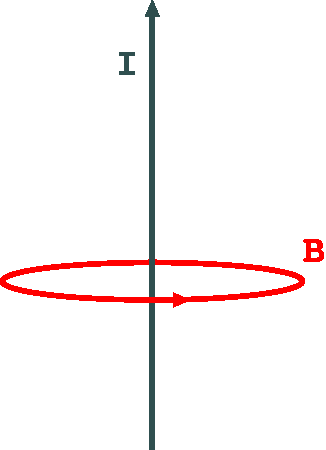
\includegraphics[height=5cm]{Ampere1.pdf} %図のファイルを指定.
  \caption{直線電流$I$の周りの磁場$B$.} %図の説明
  \label{fig:Ampere}
\end{figure} %図の終わり.
より一般的に,断面積$S$を持つ閉曲線$C$を考えると
\begin{equation}
  \frac{1}{\mu_0}\oint_C \bm{B}\cdot d\bm{l} = \int \bm{j} \cdot d\bm{S}=I
  \label{eq:integAmpere}
\end{equation}
となる.ここで,$\bm{j}$は電流密度である.

\subsection{ストークスの定理}
任意のベクトル$\bm{A}$に対して
\begin{equation}
  \int_S \bm{\nabla \times A}\cdot d\bm{S} = \oint_C \bm{A}\cdot d\bm{l}
  % 外積は\times で
  \label{eq:Stokes}
\end{equation}
が成立する。

\subsection{微分形}
ストークスの定理,式 (\ref{eq:Stokes}) を磁場$\bm{B}$に適用し,式 (\ref{eq:integAmpere})
と比較すると
\begin{equation}
  \bm{\nabla \times B} = \mu_0 \bm{j}
\end{equation}
が得られる.

\section{結論}
ガウスの法則とアンペールの法則の微分形の表式を求めた。
\begin{align} %複数行の数式を並べて表記(amsmathパッケージを利用)
  \bm{\nabla \cdot E} &= \frac{\rho_q}{\epsilon_0} \\
  \bm{\nabla \times B} &= \mu_0 \bm{j}
  %改行は \\ で行う。 & を付けた位置で各行を揃える。
\end{align}

\section*{謝辞} % *を付けると章番号が付かない.
本稿の執筆にあたり、文献\cite{fls65}を参考にした.% \cite は文献の引用.
また、文書の作成には{\LaTeX}を用いた。

\begin{thebibliography}{99} % 参考文献の始め.文献数が 100 未満なら{99}で O.K.
  \bibitem {fls65} % {}内は文献識別のため自分で付けた記号.本文で\cite{}を使うと引用できる.
  Feynman, R. P., Leighton, R. B., \& Sands, M. L., 1965, The Feynman Lectures on Physics, vol.III (ファインマン 物理学 III 電磁気学), Addison-Wesley
\end{thebibliography} %参考文献の終わり.

\end{document}